% !TeX encoding = UTF-8
% !TeX spellcheck = en_US
% !TeX root = ../../Thesis.tex

\chapter{Deflection Electronics}

\section{Demands on the setup}

For the QuaK experiment it is paramount to be able to deflect a beam of a sufficient current precisely at the right frequency with a sufficiently small bandwidth. 
As previously mentioned, our deflection system simply consists of two pairs of parallel plates between which a voltage is applied \todo[]{Optional: insert Foto of CRT's deflection plates - fig:DeflectionSetup}. Controlling this voltage allows us to control the deflection of the beam. Various aspects are important here (illustrated in \cref{fig:VoltageAspects}):

\begin{description}
	
	\item[Offset:] Although the deflection of the beam is controlled by the voltage between the plates, it is necessary to be able to set their mean potential as well. During normal operation this offset voltage is at \SI{96}{\volt} for the x-direction and at \SI{78}{\volt} for the y-direction. These offsets are necessary to keep the beam focused.
	\item[Amplitude:] The deflection coefficients in the x and y planes are \SI{19}{\volt\per\centi\meter} and \SI{11.5}{\volt\per\centi\meter} respectively (see \cite{D14363GY123-manual}). We therefore need to be able to supply up to \SI{100}{\volt} in order to be able to move the beam in a large enough area.
	\item[Frequency:] The final goal is to be able to deflect the beam at the hyperfine splitting frequency of $^{39}\mathrm{K}$, which is \SI{461.7}{\mega\hertz} or $^{41}\mathrm{K}$, with a frequency of \SI{254}{\mega\hertz}. This is likely to prove impossible with this CRT-model, observations at the highest frequency we have tried so far will be discussed in section \cref{sec:Deflection frequency}.
	\item[Waveform:] Ultimately we want the cold atoms to experience a field that oscillates like a sine wave. As a first try it is therefore reasonable to apply a sinusoidal voltage.
	\item[Lissajous curves:] Having the ability to control the deflection in both the x- and the y- axis, allows us to have our beam draw out Lissajous Curves (\cref{fig:Lissajous Curves}). By applying sine waves of equal frequency to both pairs of deflection plates and by being able to control the phase between them we can have the beam oscillate on a straight line or a circle. This allows us to generate either a linearly or circularly polarized field.
\end{description}

\begin{figure}[ht]
	\centering
		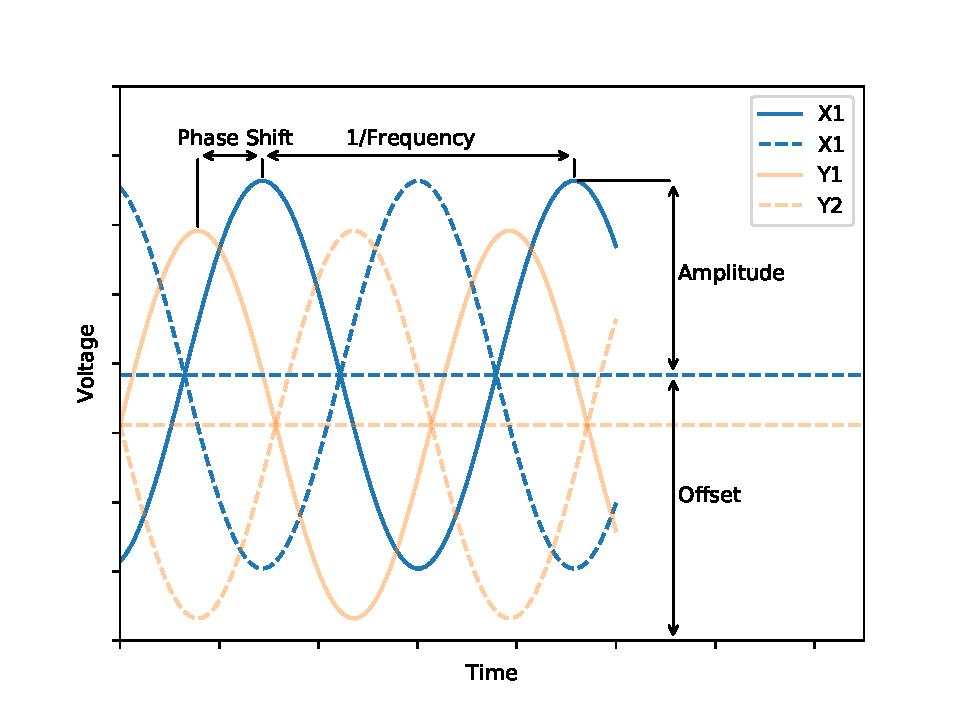
\includegraphics[width=0.7\linewidth]{Chapters/Deflection/VoltageAspects}
	\caption{}
	\label{fig:VoltageAspects}
	\todo[inline]{fr x1 to x2, caption}
\end{figure}


\begin{figure}[ht]
	\centering
	
	\begin{tikzpicture}
		% !TeX encoding = UTF-8
% !TeX spellcheck = en_US
% !TeX root = ../../Thesis.tex


\begin{groupplot}[
	group style={
		group size=5 by 1,
		horizontal sep=0mm},
	width=0.25\textwidth,
	height=0.25\textwidth]
	
	%1st plot
	\nextgroupplot[
		title={$\phi = 0$},
		xmin = -1.2, xmax = 1.2,
		ymin = -1.2, ymax = 1.2,
		xticklabels={,,},
		yticklabels={,,},
	]
	
		% phi = 0
		\addplot[
			red,
			domain=0:2*pi,
			samples=201,
		] ({sin(deg(x))}, {sin(deg(x))});

	
	
	%2nd plot
	\nextgroupplot[
	title={$\phi = \pi/4$},
	xmin = -1.2, xmax = 1.2,
	ymin = -1.2, ymax = 1.2,
	xticklabels={,,},
	yticklabels={,,},
	]
	
		% phi = pi/4
		\addplot[
			red,
			domain=0:2*pi,
			samples=201,
		] ({sin(deg(x))}, {sin(deg(x)+deg(pi/4))});
		
		
	%3rd plot
	\nextgroupplot[
	title={$\phi = \pi/2$},
	xmin = -1.2, xmax = 1.2,
	ymin = -1.2, ymax = 1.2,
	xticklabels={,,},
	yticklabels={,,},
	]
	
	% phi = pi/2
	\addplot[
	red,
	domain=0:2*pi,
	samples=201,
	] ({sin(deg(x))}, {sin(deg(x)+deg(pi/2))});
	
		
	%4th plot
	\nextgroupplot[
	title={$\phi = 3\pi/4$},
	xmin = -1.2, xmax = 1.2,
	ymin = -1.2, ymax = 1.2,
	xticklabels={,,},
	yticklabels={,,},
	]
	
	% phi = 3*pi/4
	\addplot[
	red,
	domain=0:2*pi,
	samples=201,
	] ({sin(deg(x))}, {sin(deg(x)+deg(3*pi/4))});
	
		
	%5th plot
	\nextgroupplot[
	title={$\phi = \pi$},
	xmin = -1.2, xmax = 1.2,
	ymin = -1.2, ymax = 1.2,
	xticklabels={,,},
	yticklabels={,,},
	]
	
	% phi = pi
	\addplot[
	red,
	domain=0:2*pi,
	samples=201,
	] ({sin(deg(x))}, {sin(deg(x)+deg(pi))});
	
		
	
\end{groupplot}
	\end{tikzpicture}
	
	\caption{Lissajous Curves}
	\label{fig:Lissajous Curves}
\end{figure}

\section{Implementation}

\begin{figure}[ht]
	\centering
	
	\begin{tikzpicture}
		% !TeX encoding = UTF-8
% !TeX spellcheck = en_US
% !TeX root = ../../Thesis.tex

\ctikzset{sources/scale=0.5}
\ctikzset{transformer L1/.style={inductors/coils=6}, transformer L2/.style={inductors/coils=6}}  % set coil number so that midtap touches coil

\newcommand{\coaxial}[2] % coordinates of left inner wire, length of cable
% draw a coaxial cable with given length
{
	\draw (0 + {#1}[0], {#1}[1]) to[short, -] (#2 + {#1}[0], {#1}[1]); % middle line
	\draw (0.5 + {#1}[0], 0.25 + {#1}[1]) -- (#2 - 0.5 + {#1}[0], 0.25 + {#1}[1]); % top line
	\draw (0 + {#1}[0], -0.25 + {#1}[1]) to[short, -] (#2 + {#1}[0], -0.25 + {#1}[1]); % bottom line
	\draw (0.5 + {#1}[0], {#1}[1]) circle [radius=0.25]; % left circle
	\draw (#2 - 0.5 + {#1}[0], {#1}[1]) circle [radius=0.25]; % right circle
}

%\draw [help lines] (0, 0) grid (15, 12);
%\filldraw (0, 0) circle (0.5mm);


% signal generator
\draw (0, 3) rectangle (2, 4) node [midway]{RF};
\coaxial{2, 3.5}{2}
\draw (4, 3.25) node [ground] {};
\draw (4, 3.5) to ++ (1, 0);

% x signal
\draw (5, 3.5) to ++ (0, 1.5) to ++ (2, 0) to [twoport, t=AMP] ++ (2, 0) node [transformer, anchor=A1] (x-transformer) {};
\draw (x-transformer.A2) node [ground] {};  % gound left side
\draw (x-transformer.B1) to ++ (2, 0) node [right] {x1}; % connection to x1
\draw (x-transformer.B2) to ++ (2, 0) node [right] {x2}; % connection to x2
\draw (x-transformer-L2) to [dcvsource, label=\SI{96}{\volt}] ++ (2, 0) node [ground] {};  % bias center to ground

% y signal
\draw (5, 3.5) to ++ (0, -2) to [vphaseshifter] ++ (2, 0) to [twoport, t=AMP]++ (2, 0) node [transformer, anchor=A1] (y-transformer) {};
\draw (y-transformer.A2) node [ground] {};  % gound left side
\draw (y-transformer.B1) to ++ (2, 0) node [right] {y1}; % connection to y1
\draw (y-transformer.B2) to ++ (2, 0) node [right] {y2}; % connection to y2
\draw (y-transformer-L2) to [dcvsource, label=\SI{78}{\volt}] ++ (2, 0) node [ground] {};  % bias center to ground

	\end{tikzpicture}
	\caption{Deflection circuit.}
	\label{fig:deflec_circuit}
\end{figure}

A first setup with which we can try to obtain the desired voltages is depicted in \cref{fig:deflec_circuit}. On the  very left we have a signal generator that is capable of producing the right frequency (\SI{461.7}{\mega\hertz}) this signal is then split up into an x-, and a y-branch. One of the two branches is connected to a phase shifter, which is able to delay the input signal by up to \SI{200}{\degree}, allowing us to set any desired phase shift between x-, and y-deflection and to correct for inadvertent delays from the other electronics. Both the x-, and  y-signal are then amplified using (amplifier) \todo[]{Find out which amplifier}. In the final step, a center tapped transformer allows us to produce voltages for the plates X1 and X2 (or Y1 and Y2 respectively) with a phase shift of exactly \SI{180}{\degree} between them. By setting the center tap to the desired offset potential, we should get the voltage curves described above. To understand this setup in more detail, it is useful to examine its most important parts more closely:

\begin{description}
	\item[Amplifier:] Up to now we have used the XXX \todo[]{which model?} and the YYY \todo[]{which model?} amplifier, which have a fixed gain of (How much?) \todo[]{Check amplifier specifications}. Inputs and outputs can simply be connected via BNC cables. The amplifier is powered by a linear power supply with a DC voltage of \SI{24}{\volt} via two banana plugs in the front. Since we want to control the Lissajous curves shapes (as the deflection coefficients for the x- and y- plates differ), it is desirable to be able to adjust the amplifier gain in future versions of the setup. 
	
	\item[Center Tapped Transformer:] The center tapped transformer we use is the Mini-Circuits TC8-1G2+ (\cite{TC8-1G2}), a transformer for frequencies between \SIrange{2}{500}{\mega\hertz}, with an impedance ratio of 8. \Cref{fig:CTT} shows how the center tapped transformer is implemented. The in- and outputs, as well as the bias voltage can be connected via BNC cables. As usual, the shields of all these cables are connected to ground, furthermore they are connected to each other and to the housing. As a safety feature, both outputs X1 and X2 are directly connected to the bias through an arrangement of diodes: Two connections, each with a normal diode and a Zener diode facing in opposite directions. The breakthrough voltage of the Zener diode is \SI{200}{\volt}, during normal operation the voltage on it stays below this value and none of the connections let any current through as one of the two diodes is always blocking it. However if one of the plates in the CRT accidentally comes in contact with high voltage, the connection with the appropriately oriented Zener diode opens up, preventing a voltage spike on the center tapped transformer and thereby protecting the electronics connected to its primary circuit.
	At the point of writing there are still some problems with the behavior of the center tapped transformer, the capacitance of the diodes introduces an undesired phase shift between the two signals. \Cref{fig:unbiased2} shows the circuit's behavior at \SI{465}{\mega\hertz} without its diodes, here the signals are shifted by $\SI{120}{\pico\second} \mathrel{\widehat{=}} \SI{20}{\degree} = \SI{0.35}{\radian}$. Additionally, applying a bias voltage leads to differing amplitudes, as can be seen in \cref{fig:biased2}.
	
	\item[Phase Shifter:] To control the phase shift between the x- and y-deflection plates, we use a Mini-Circuits \cite{JSPHS-661} phase shifter. This part was put in a  housing (\cite{Hammond1455D601RD}) on a separate PCB and can be connected via BNC cables. \Cref{fig:circuit_phase} shows how the phase shifter is connected and \cref{fig:PCB_phase} shows the corresponding PCB layout. Note that again the shields of the BNC cables are connected among each other and to the housing. The JSPHS-661+ is designed for frequencies in the range \SIrange{400}{600}{\mega\hertz}. By applying a DC voltage of \SIrange{0}{12}{\volt} to the bias connector, it is possible to introduce a phase shift of up to \SI{200}{\degree} to the signal.
	
\end{description}

(figure)\todo[]{Insert fotos of finished circuits in housings}\\

\begin{figure}[ht]
	\centering
	\begin{subfigure}{0.4\textwidth}
		\centering
		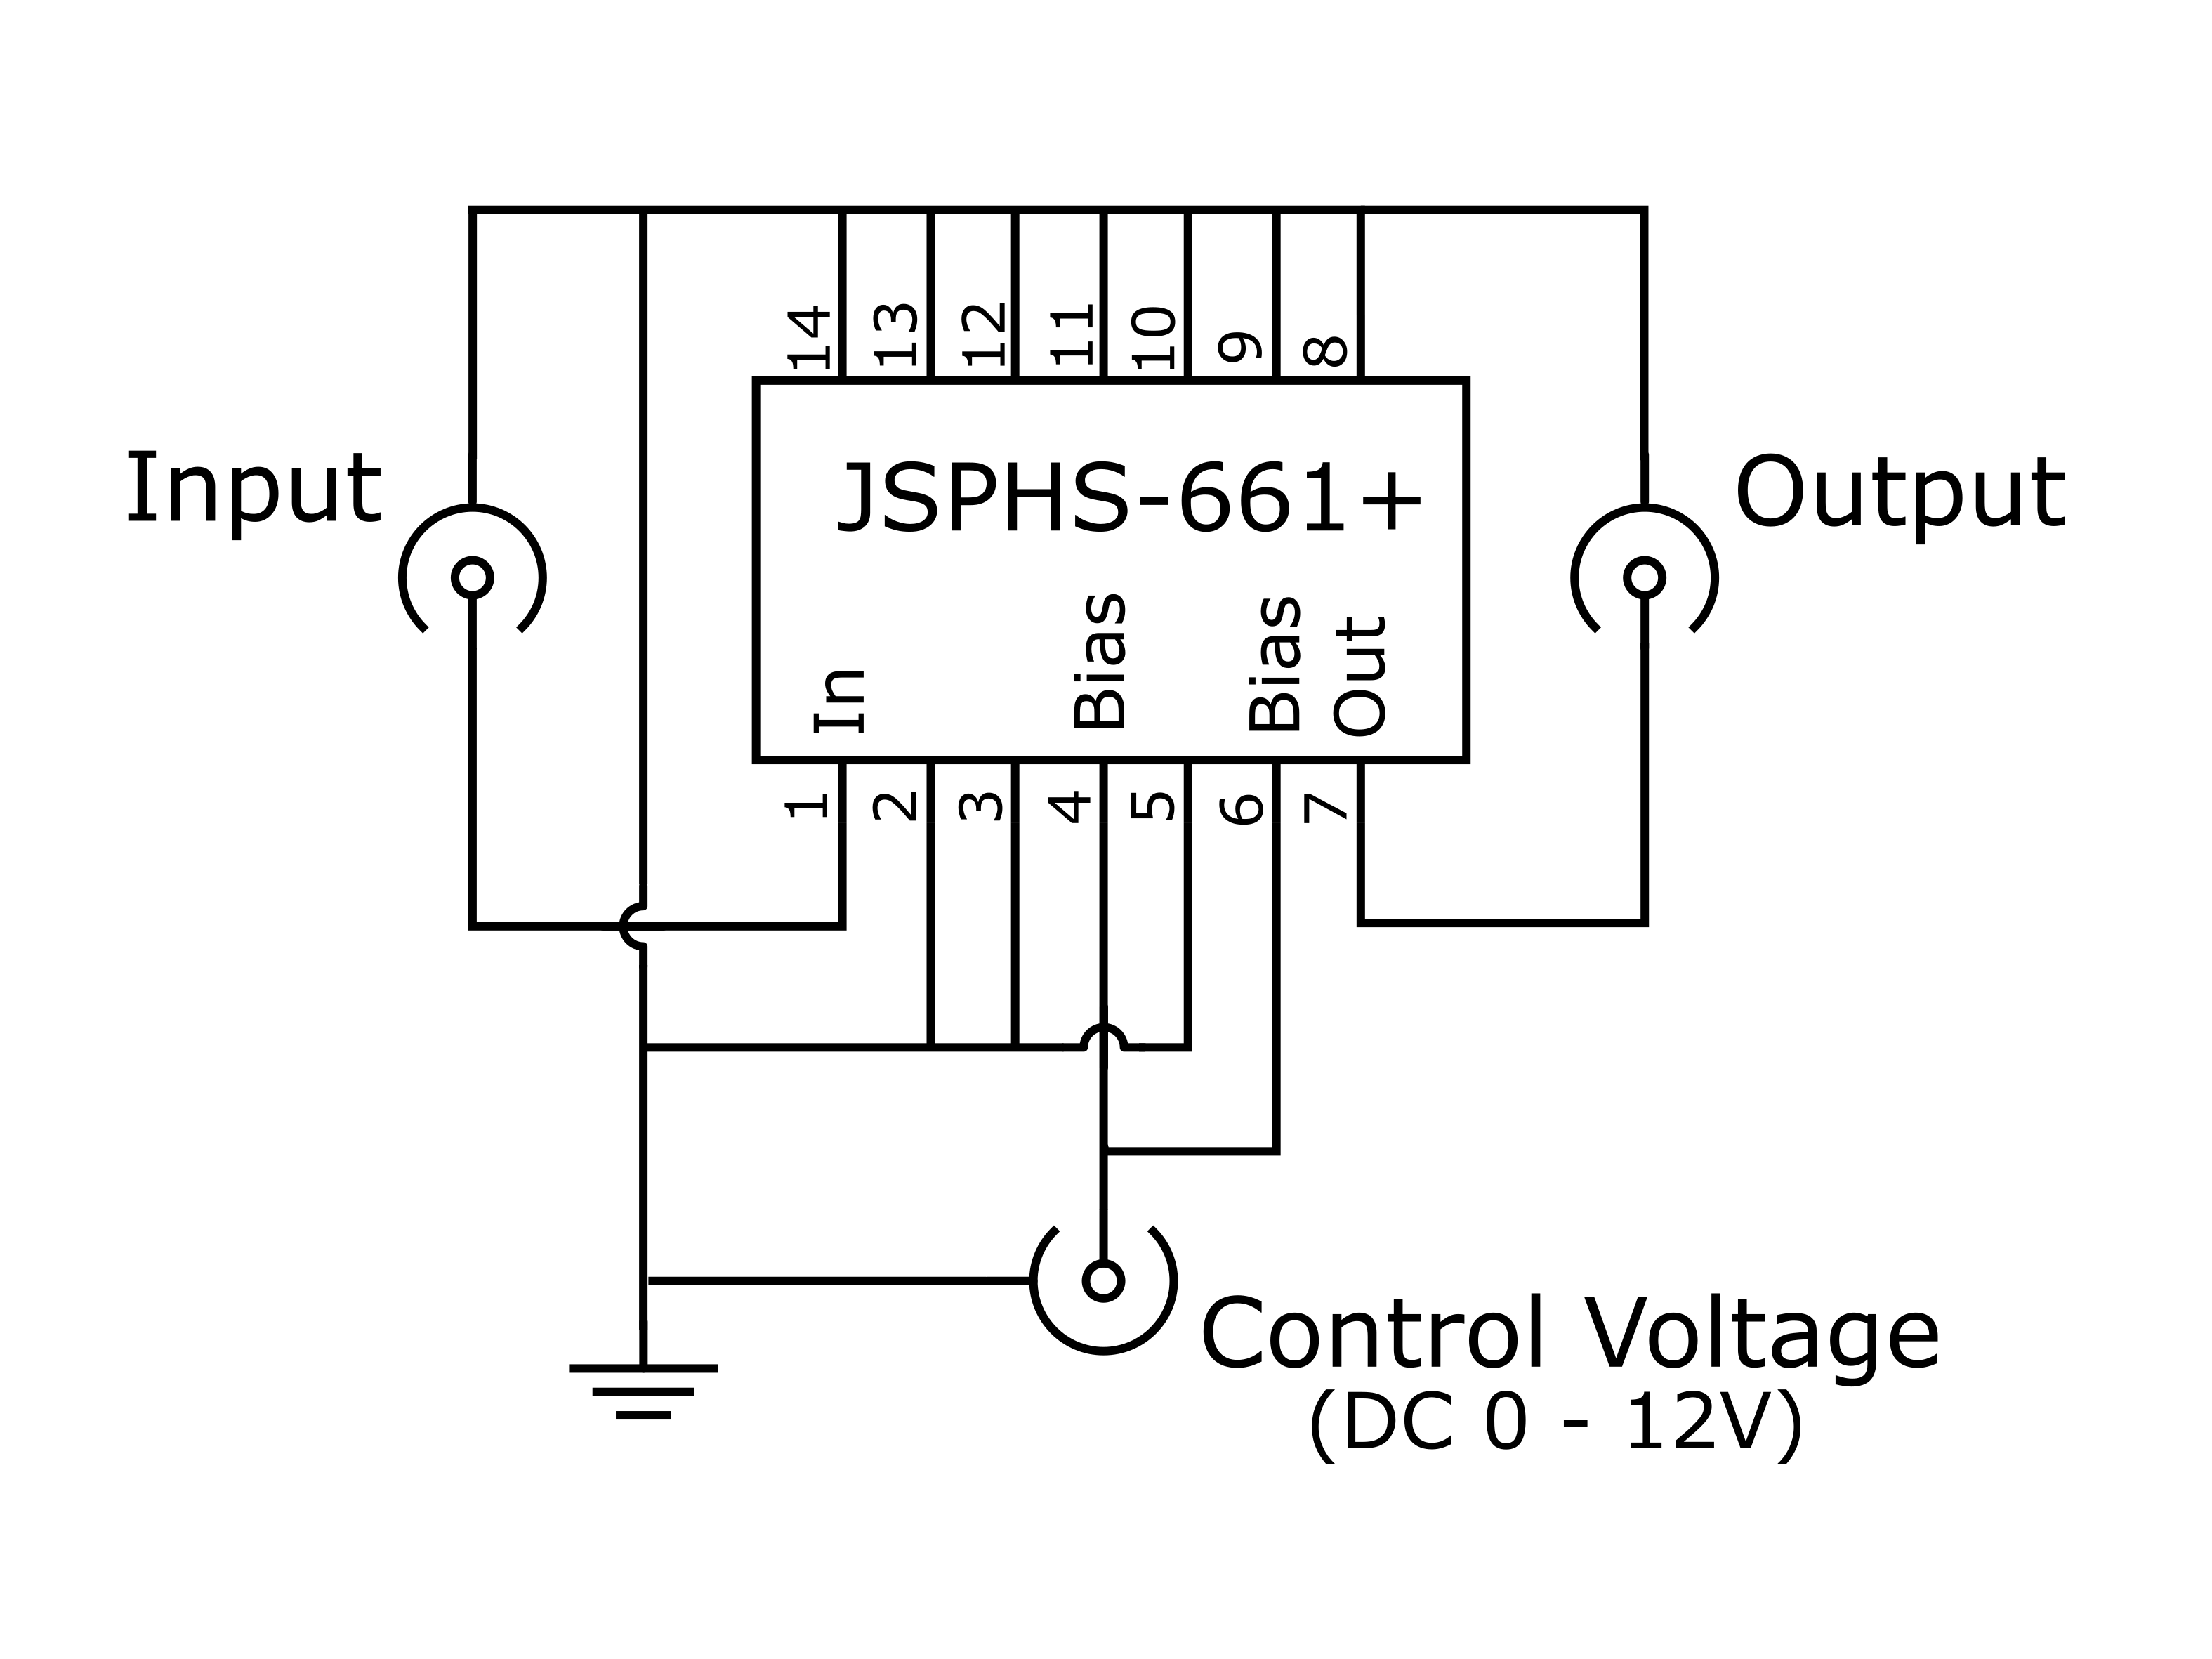
\includegraphics[width=\textwidth]{Chapters/Deflection/circuit_phase4zu3}
		\caption{Schematic of phase shifter connections}
		\label{fig:circuit_phase}
	\end{subfigure}
	\hspace{0.1\textwidth}
	\begin{subfigure}{0.4\textwidth}
		\centering
		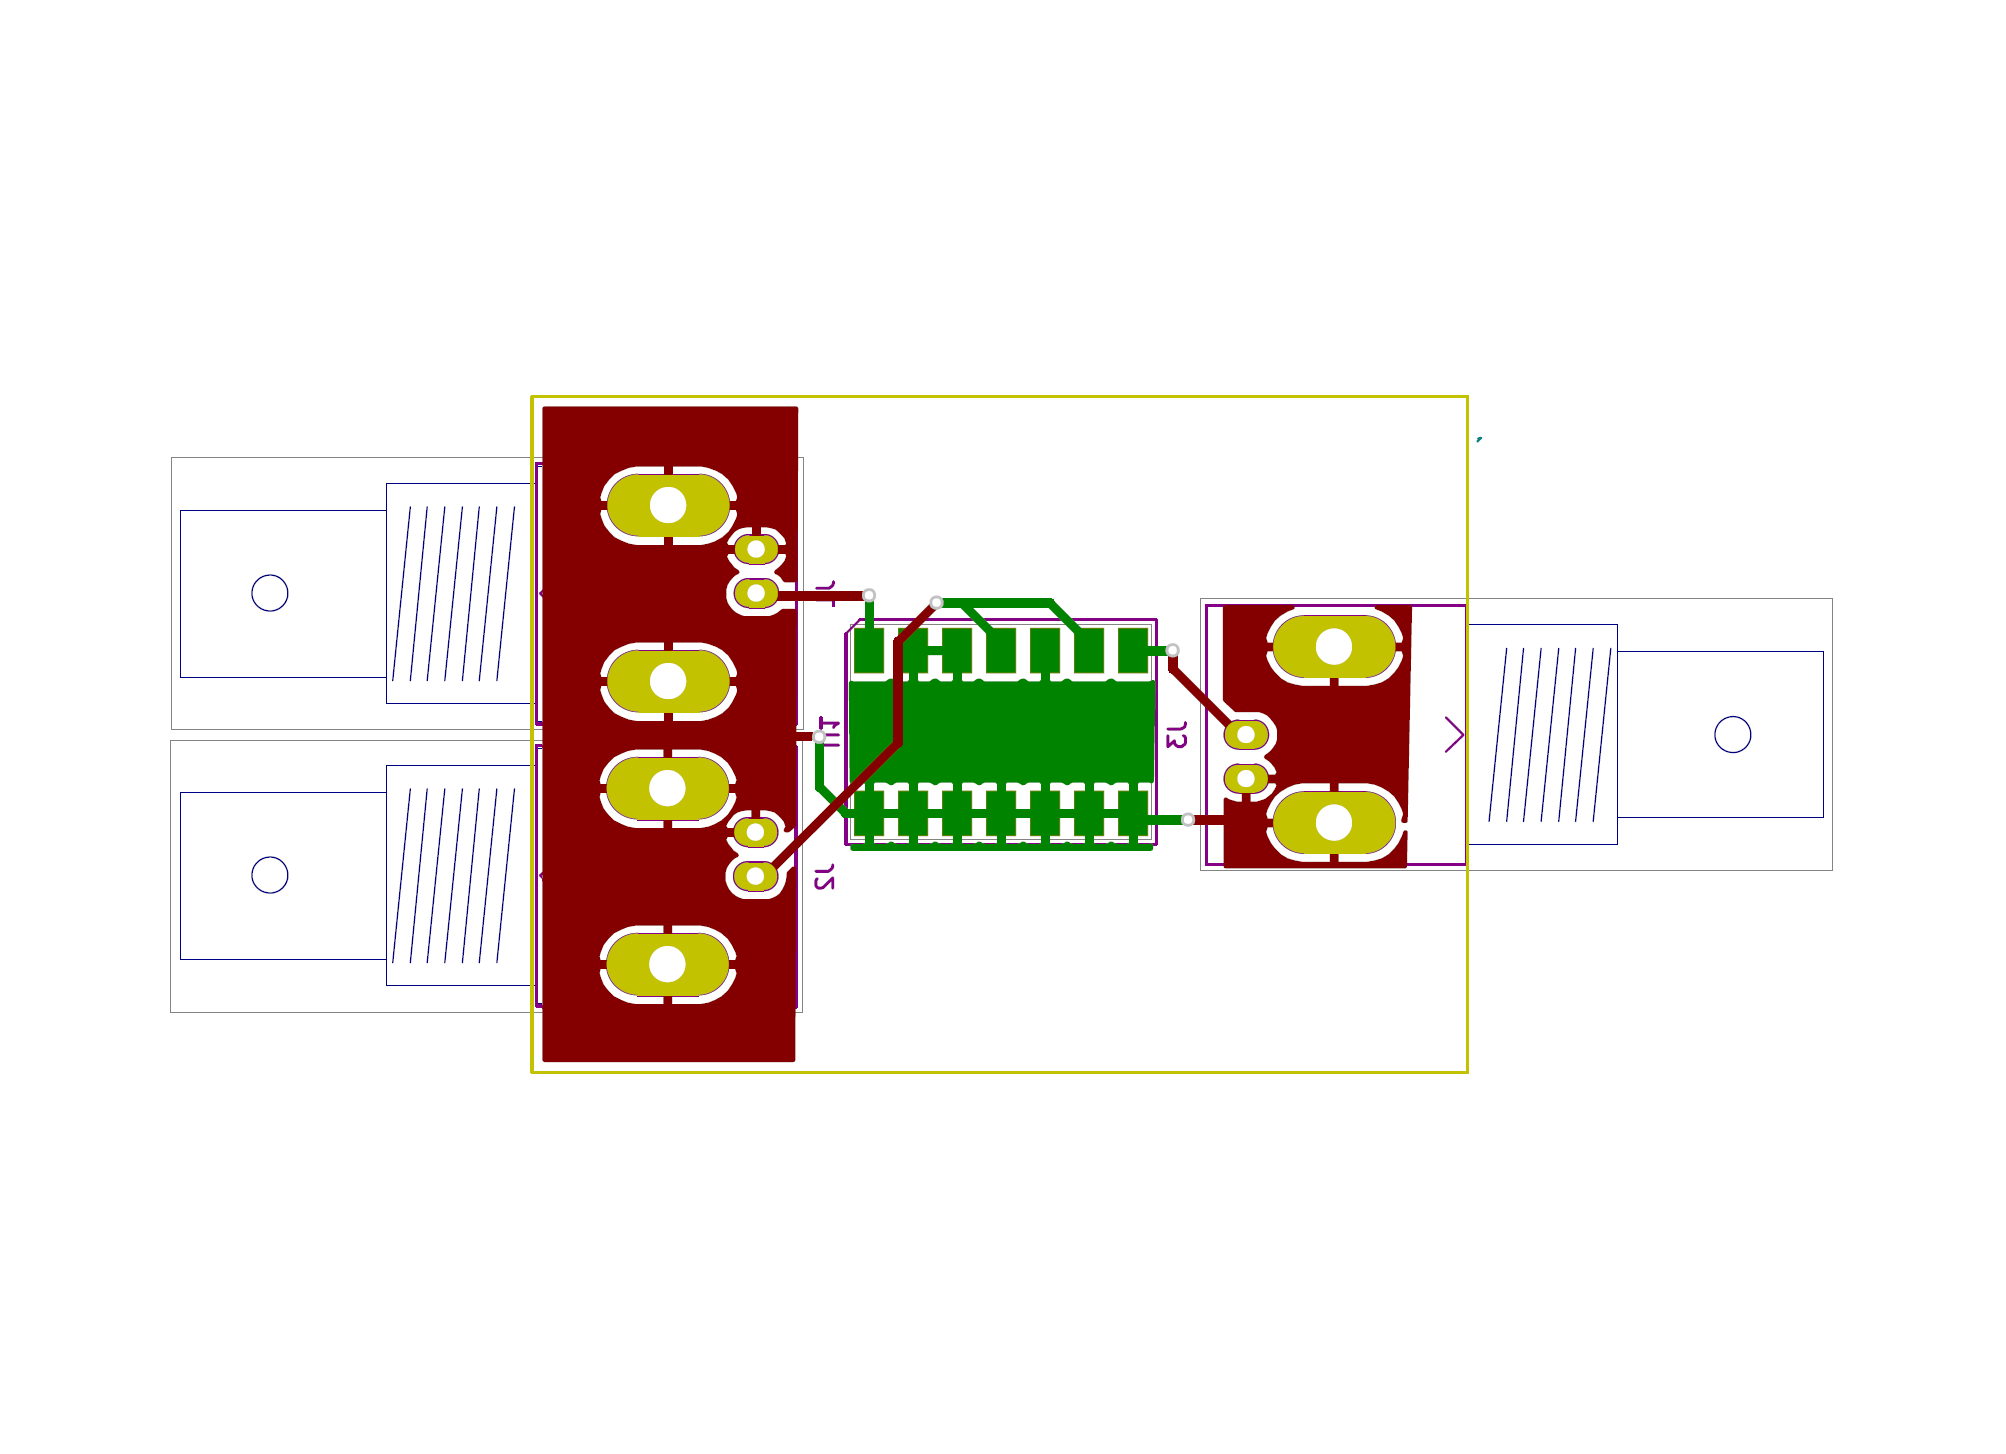
\includegraphics[width=\textwidth]{Chapters/Deflection/PCB_phase3}
		\caption{PCB-Layout of the phase shifter}
		\label{fig:PCB_phase}
	\end{subfigure}
	\caption{}
	\label{fig:PhaseShifter}
\end{figure}




\begin{figure}[ht]
	\centering
	\begin{subfigure}{0.4\textwidth}
		\centering
		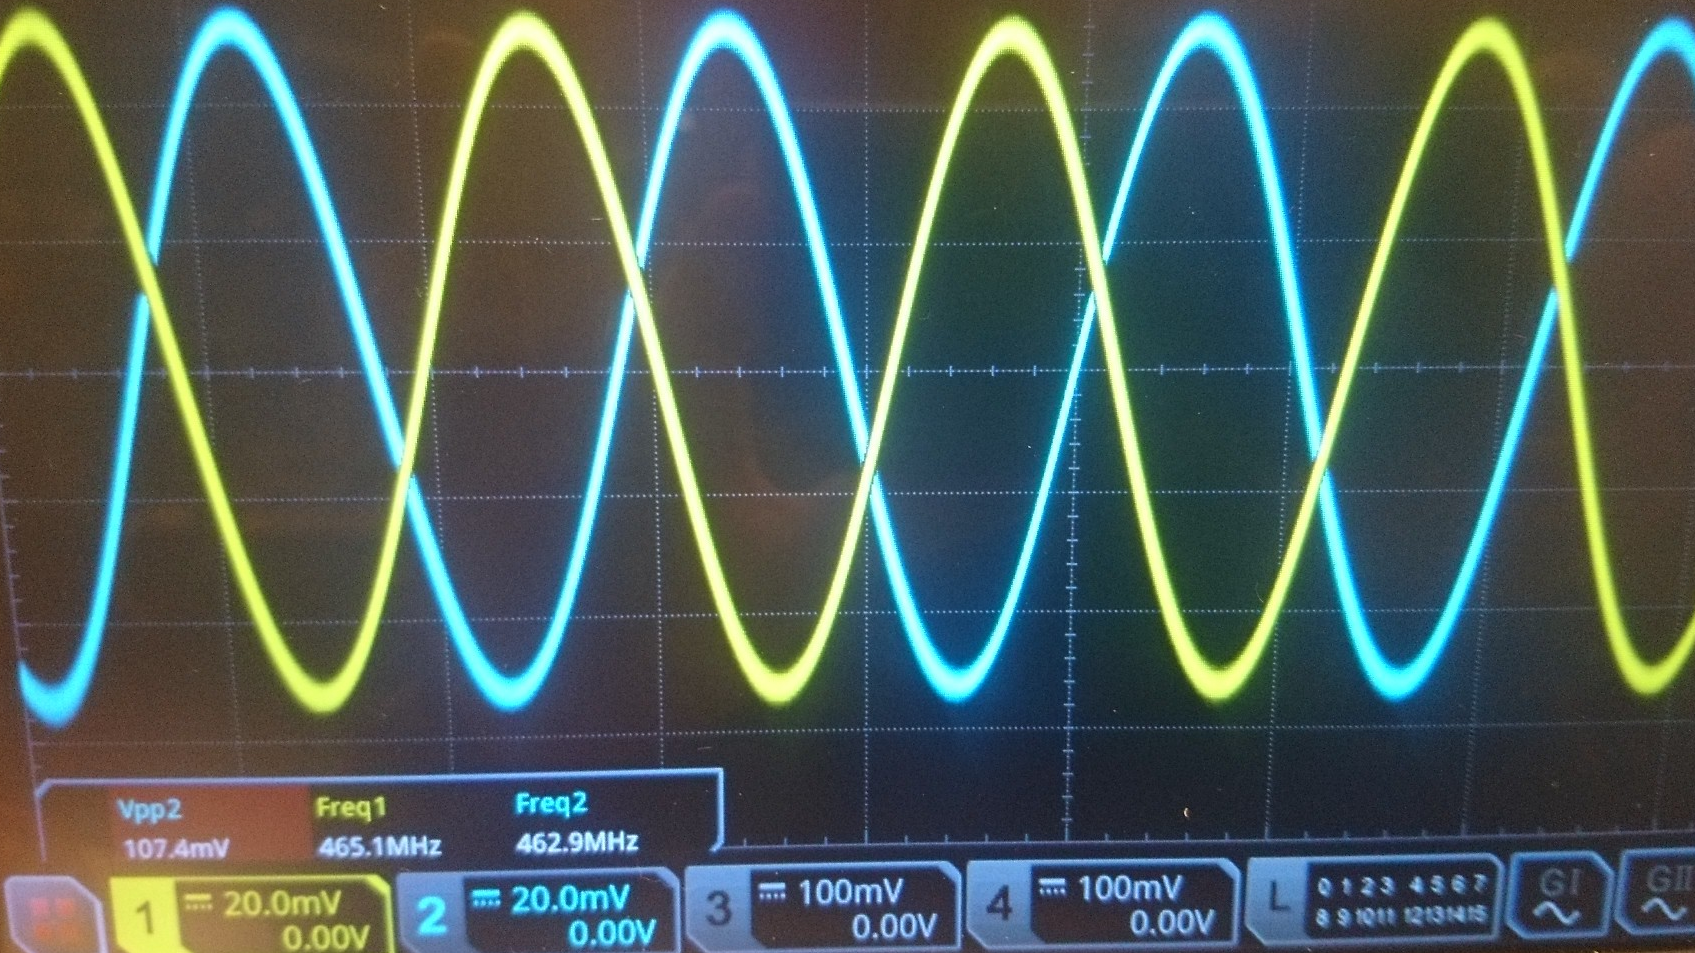
\includegraphics[width=\textwidth]{Chapters/Deflection/unbiased3}
		\caption{Signal of center tapped transformer without diodes, unbiased at \SI{465}{\mega\hertz}}
		\label{fig:unbiased2}
	\end{subfigure}
	\hspace{0.1\textwidth}
	\begin{subfigure}{0.4\textwidth}
		\centering
		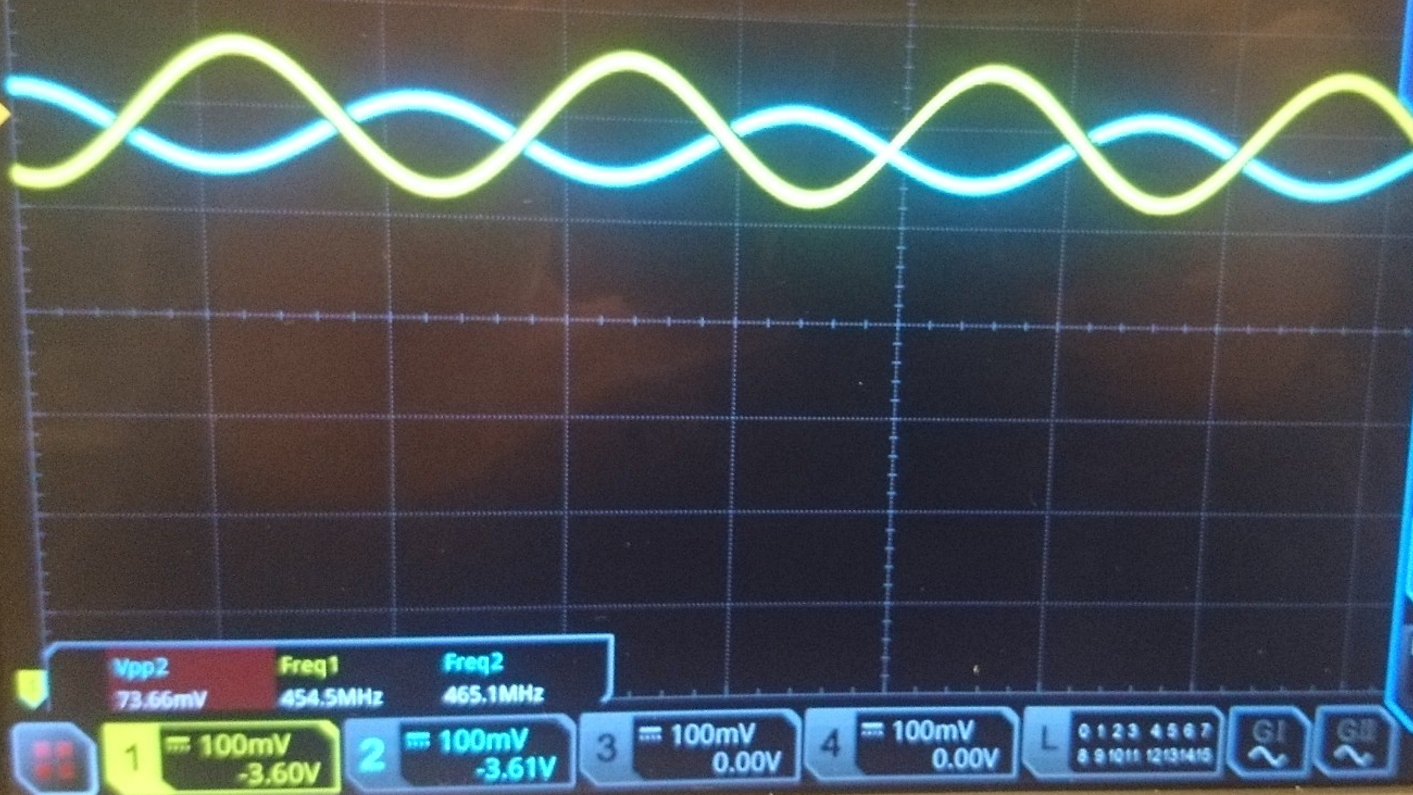
\includegraphics[width=\textwidth]{Chapters/Deflection/biased3}
		\caption{Signal of center tapped transformer without diodes, biased at \SI{465}{\mega\hertz}}
		\label{fig:biased2}
	\end{subfigure}
	\caption{}
	\label{fig:CTTSignal}
\end{figure}



\begin{figure}[ht]
	\centering
	\begin{subfigure}{0.4\textwidth}
		\centering
		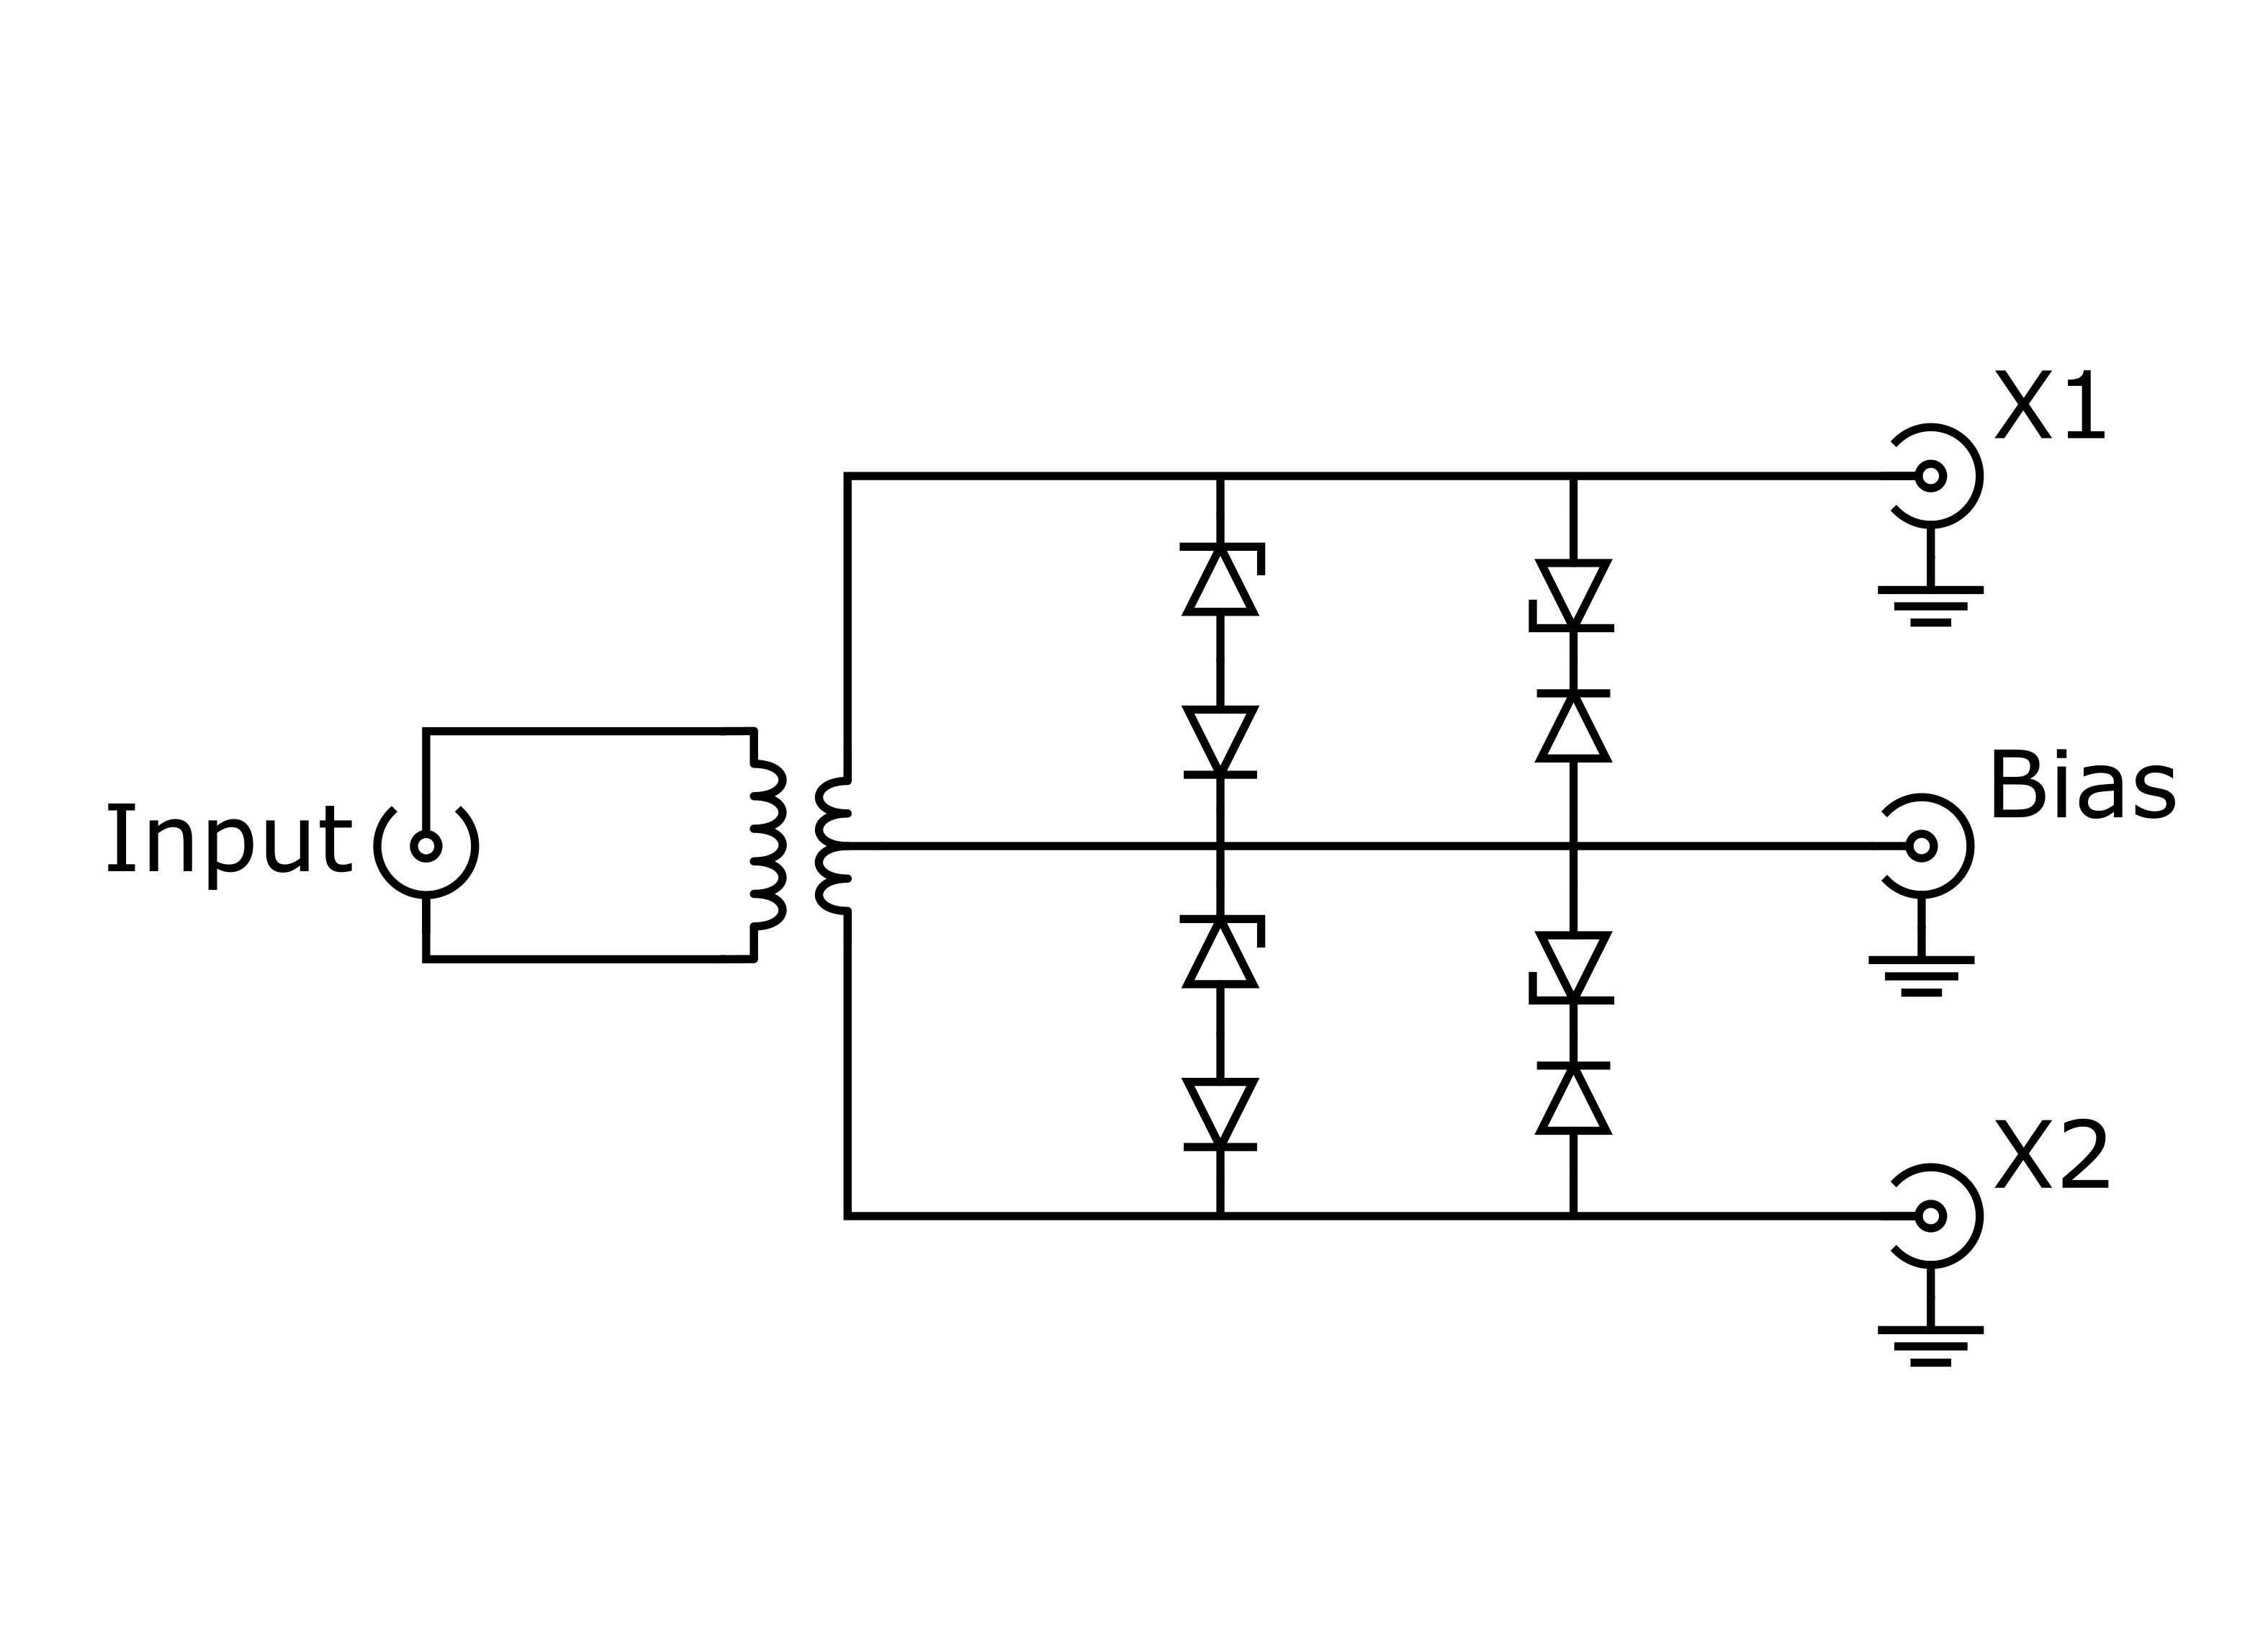
\includegraphics[width=\textwidth]{Chapters/Deflection/circuit_CTT4zu3}
		\caption{Schematic of center tapped transformer connections}
		\label{fig:circuit_ctt}
	\end{subfigure}
	\hspace{0.1\textwidth}
	\begin{subfigure}{0.4\textwidth}
		\centering
		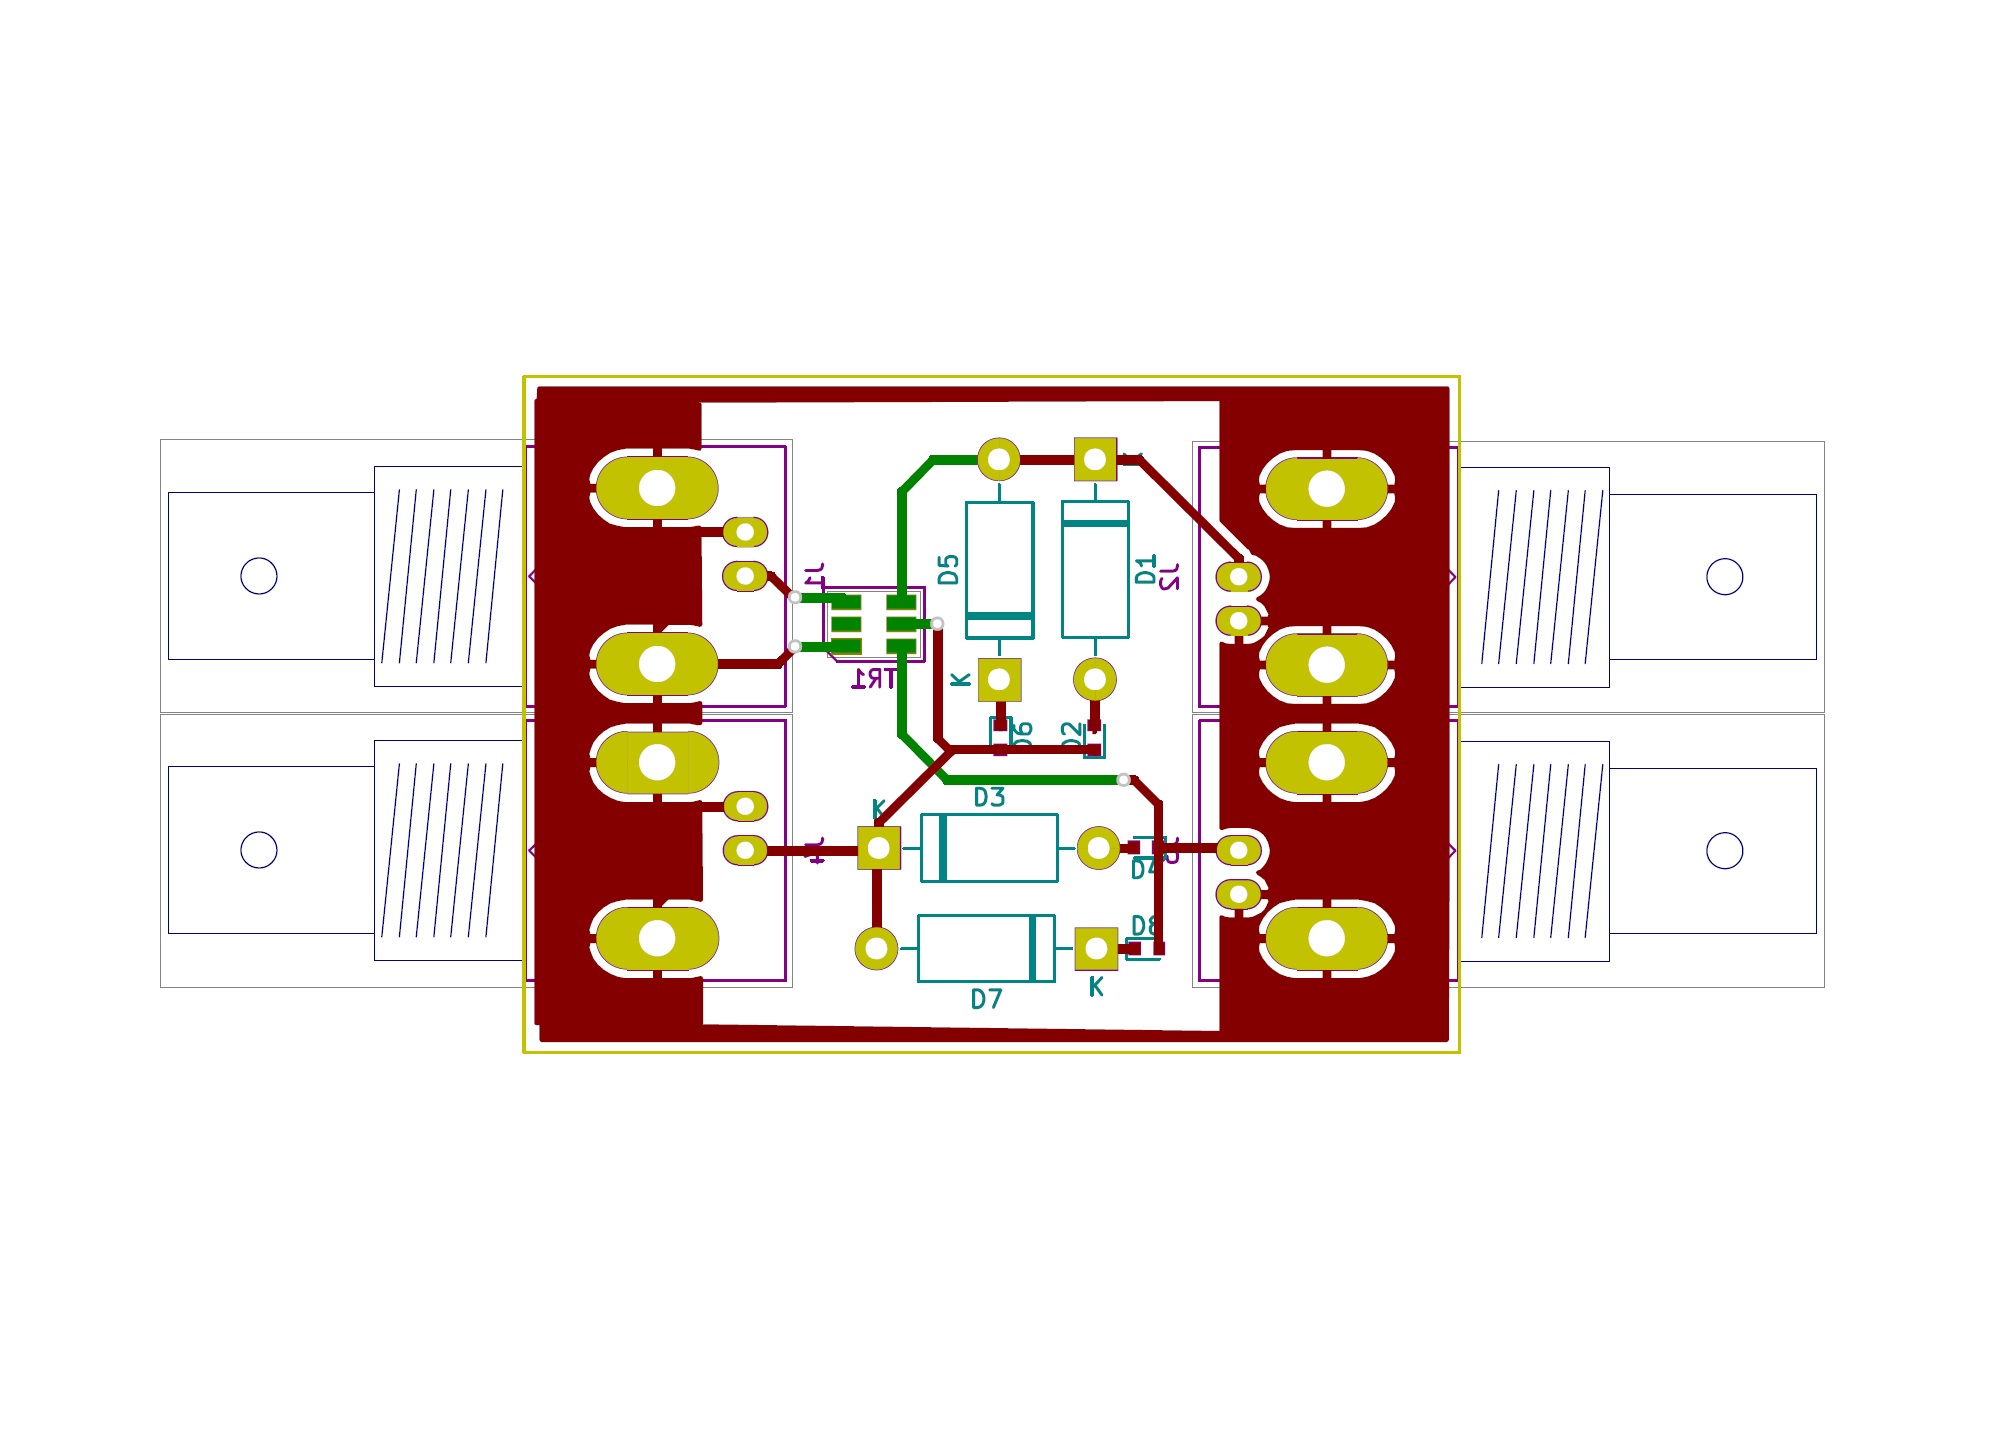
\includegraphics[width=\textwidth]{Chapters/Deflection/PCB_CTT3}
		\caption{PCB-Layout for center tapped transformer}
		\label{fig:PCB_CTT}
	\end{subfigure}
	\caption{}
	\label{fig:CTT}
\end{figure}

\todo{Einheiten hinschreiben}


